\documentclass[11pt,a4paper]{jarticle}
\usepackage[dvipdfmx]{graphicx}
\usepackage{url}

\renewcommand{\baselinestretch}{1.05} 
\marginparwidth=0cm
\topmargin=-1cm
\headheight=0.3cm
\headsep=0.7cm
\oddsidemargin=0cm
\evensidemargin=0cm
%\textwidth=43zw
\textwidth=15.92cm
%\textheight=43.3\baselineskip
\baselineskip = 0.5744cm
\textheight=43\baselineskip

\itemsep=0.05\baselineskip
\parsep=0pt
\topsep=0.01\baselineskip
\partopsep=0pt
\listparindent=0zw

%% header and footer
\usepackage{fancyhdr}
\pagestyle{fancy}
\lhead{2014 年 4 月 x 日} % 日にち変える
\chead{インタラクティブ・アート実習}
\rhead{担当教員: 松下 光範}
\cfoot{\thepage}
\renewcommand{\headrulewidth}{0pt}
\renewcommand{\footrulewidth}{0pt}

\usepackage{ascmac}
\usepackage{listings,jlisting}
\usepackage{color}
\definecolor{OliveGreen}{cmyk}{0.64,0,0.95,0.40}
\definecolor{colFunc}{rgb}{1,0.07,0.54}
\definecolor{CadetBlue}{cmyk}{0.62,0.57,0.23,0}
\definecolor{Brown}{cmyk}{0,0.81,1,0.60}
\definecolor{colID}{rgb}{0.63,0.44,0}
\definecolor{rulesepcolor}{gray}{0.666}
\lstset{
  language=Java,%プログラミング言語によって変える。
  numbers=left,
  basicstyle={\ttfamily\small},
  keywordstyle={\color{OliveGreen}},
  %[2][3]はプログラミング言語によってあったり、なかったり
  keywordstyle={[2]\color{colFunc}},
  keywordstyle={[3]\color{CadetBlue}},%
  commentstyle={\color{Brown}},
  %identifierstyle={\color{colID}},
  stringstyle=\color{blue},
  tabsize=2,
  %frame=trBL,
  %numbers=left,
  numberstyle={\ttfamily\small},
  breaklines=true,%折り返し
  %backgroundcolor={\color[gray]{.95}},
  framexleftmargin=0mm,
  frame=shadowbox,
  rulesepcolor=\color{rulesepcolor},
  captionpos=b
}


%%%%%%%%%%%%%%%%%%%%%%%%%%%%%%%%%%%%%%%%%%%%%%%%%%%%%%%%%%%%%%%%
\begin{document}

% title
\section*{\LARGE{第2講 プログラムと I/O モジュールを組み合わせる}}
プログラミング言語「Processing」と「Arduino」を組み合わせる。

%%%%%%%%%%%%%%%%%%%%%%%%%%%%%%%%%%%%%%%%%%%%%%%%%%%%%%%%%%%%%%%%


\section{Processing とは}
Processing\footnote{\url{http://processing.org/}} は、Casey Reas と Benjamin Fry によるオープンソースプロジェクトであり、かつてはMITメディアラボで開発されていた。
電子アートとビジュアルデザインのためのプログラミング言語であり、統合開発環境 (IDE) である。 視覚的なフィードバックが即座に得られるため、初心者がプログラミングを学習するのに適しており、電子スケッチブックの
基盤としても利用できる。
Javaを単純化し、グラフィック機能に特化した言語といえる。

\begin{flushright}
 -wikipedia-
\end{flushright}

\subsection*{Processing の開発環境}
Processing のアイコンをダブルクリックすると、統合開発環境 (IDE) が立ち上がる。

\begin{figure}[h]
 \centering
 \includegraphics[width=0.5\columnwidth]{img/processing_ide.eps}
 \caption{Processing の統合開発環境}
\end{figure}


\section{Processing によるプログラミング}
以下で、Processing による基本的なプログラミングの説明を行います。
なお、メニューバーの「Help → Reference」でインターネットブラウザが起動し、より詳しい説明が確認できますので、そちらも参考にしてください。
ただし、英語表記です。
Processing にはあらかじめサンプルコード (お手本になるプログラム) が、たくさん用意されているので、それを動かしてみてどんなことができるかを見ておくのも良いかもしれません。
サンプルコードは、メニューバーの「File → Example」から見ることができます。

\subsection*{基礎となるプログラム}

\begin{lstlisting}
 void setup() {
   // プログラム開始時に一度だけ実行
 }

 void draw() {
   // setup() の後、プログラムが終わるまで繰り返される
 }
\end{lstlisting}


% \section{code test}

% \begin{lstlisting}
% import processing.gainer.*;

% Gainer gainer; 

% void setup() {
%   size(400, 400);

%   // Gainer の Analog Input を使う準備
%   gainer = new Gainer(this);
%   gainer.beginAnalogInput();
% }
 
% void draw() {
%   // Analog Input の 0 番ポートに繋がれているセンサの値を取得
%   int value = gainer.analogInput[0];

%   println(value);
% }
% \end{lstlisting}
% % 別ファイルを読み込む場合
% % \lstinputlisting[caption=キャプション,label=ラベル]{プログラムまでのパス}

\end{document}